\documentclass[a4,12pt]{horizon-theme}
\usepackage{lipsum}
\usepackage{fontawesome5}
\usepackage{graphicx,url}
\usepackage{float}
\usepackage{amsmath}
\usepackage{booktabs}
\usepackage{makecell}
\usepackage{array}
\usepackage{multirow}
\usepackage{caption}
\usepackage{subcaption}
\usepackage{siunitx}
\usepackage{enumerate}
\usepackage{gensymb}
\usepackage{csvsimple}
% \usepackage{tabularray}
\usepackage{stackengine}
\usepackage{xcolor, colortbl}
\usepackage{caption}
\usepackage[round]{natbib}
\usepackage[thinc]{esdiff}
% \usepackage{longtable}


\strutlongstacks{T}

\setFiguresPath{.}
\setTitle{Modelagem de um Sistema de Resfriamento de Chips}
\setUniversity{Universidade de São Paulo}
\setFaculty{Escola Politécnica}
\setDepartment{MAP3121 - Métodos Numéricos e Aplicações}
\setCoverMainLogo{minerva.pdf}

\setCoverLeftBox{%
  {\Large Exercício Programa 03}\\[2pt]
  {Relatório Final}\\[45pt]
  {\large Natanael Magalhães Cardoso, 8914122}\\[5pt]
  {\large Valber Marcelino Filho, 11353165}\\[40pt]
  {\normalsize Professora: }{\large Cláudia Peixoto}\\[5pt]
  {\normalsize Turma: }{\large 03}
}

\renewcommand{\thefootnote}{\fnsymbol{footnote}}
\setCompactAuthors{Natanael Magalhães Cardoso\footnote{nUSP: 8914122, Turma: 03}, Valber Marcelino Filho\footnote{nUSP: 11353165, Turma: 03}}


\setHeaderRight{Escola Politécnica}
\setHeaderLeft{MAP3121 - Métodos Numéricos e Aplicações}



\begin{filecontents*}{a_n5_d4.csv}
i,a,b,c,d,x
1,{\bf 0.0000},2.0000,0.7500,0.9686,0.3827
2,0.3750,2.0000,0.6250,0.5358,0.2709
3,0.4167,2.0000,0.5833,-0.6374,-0.2392
4,0.4375,2.0000,0.5625,-0.6374,-0.4660
5,0.9000,2.0000,{\bf 0.0000},1.0000,0.7097
\end{filecontents*}


\DeclareUnicodeCharacter{2212}{-} % fix

\begin{document}
\horizonCover

\horizonTitle

\renewcommand{\thefootnote}{\arabic{footnote}}
\hspace{40pt}


\section{Introdução}

O método de Rayleigh-Ritz é usado para obtenção de resultados aproximados para equação diferencial parcial dadas as condições de contorno. Neste método, o problema de valor limite é primeiramente formulado para um problema de escolha. Entre todo o conjunto de funções diferenciáveis que satisfazem as condições de limite, escolhe-se as funções que minimizam uma certa integral. Então, o conjunto de funções viáveis fica reduzido, para resultar em uma solução para o problema de minimização e, consequentemente, numa solução para o problema de valor limite.

O método de Rayleigh-Ritz é comumente utilizado para obter uma solução para o modelo da viga de Euler-Bernoulli (biapoiada) com rigidez de flexão constante, ou seja, mesmo material e mesma seção transversal em todo o domínio. Em certas áreas da engenharia, como mecânica e civil, são utilizadas estruturas como vigas, treliças e placas que possuem propriedades necessárias para a construção de prédios, aviões e navios. Essas estruturas estão sujeitas a cargas de tração, torção, flexão. Sendo assim, elas precisam ser projetadas para suportar essas forças, permitindo que possam exercer suas funções sem problemas.

Neste projeto, utilizaremos o método de Rayleigh-Ritz com aproximação por splines lineares para modelar numericamente um sistema termodinâmico conservativo: o comportamento da difusão térmica que ocorre em um chip sujeito a aquecimento e sob ação de um resfriador.


\newpage
\section{Métodos}
\label{sec:metodo}

\subsection{Modelagem do sistema termodinâmico}
\label{sec:modelagem}

Este problema será restrito à análise unidimensional e a distribuição de calor pode é modelada pela equação do calor obtida a partir da lei de Fourier e da propriedade de conservação de energia

\begin{equation}\label{eq:termo}
  \rho C\frac{\partial T}{\partial t}\left(t,x\right)=\frac{\partial }{\partial x}\left(k\left(x\right)\frac{\partial T}{\partial x}\left(t,x\right)\right)+Q\left(x\right)
\end{equation}
onde $T(t, x)$ é a temperatura do processador no instante $t$ e na posição $x$; $\rho$ é a densidade do material; $C$ é o calor específico do material; $k$ é a condutividade térmica e $Q$ é uma fonte de calor.

Do ponto de vista elétrico, a potência dissipada por um circuito integrado ($P$) pode ser expressa pela eq. \eqref{eq:pot}.

\begin{equation}\label{eq:pot}
  P = C \cdot V^2 \cdot f
\end{equation}
onde $C$ é a capacitância parasita, $V$ é a tensão de alimentação e $f$ é a frequência de clock

No caso real, a potência sofre variações, pois a tensão pode oscilar, bem como a frequência, que depende da carga de trabalho. Contudo, nesta análise será considerando um processador que trabalhe em regime constante, gerando sempre a mesma quantidade de calor e que o resfriador sempre consiga extrair a mesma quantidade de calor. Isso implica em uma taxa de variação da temperatura no tempo nula, como expressa a eq. \eqref{eq:constante}

\begin{equation}\label{eq:constante}
  \frac{\partial T}{\partial t}\left(t,x\right)=0
\end{equation}

Então, a eq. \eqref{eq:termo} pode ser simplificada para eq. \eqref{eq:estacionario}

\begin{equation} \label{eq:estacionario}
  -\diffp{}{x}\left(k(x)\diffp{T(x)}{x}\right) = Q(x)
\end{equation}

Com o equacionamento do sistema físico a ser estudado completo, desejamos obter a solução de equilíbrio resolvendo numericamente a equação (\ref{eq:estacionario}) usando o método dos elementos finitos.


\subsection{Método de Rayleigh-Ritz}
\label{sec:rr}

O método de Rayleigh-Ritz fornece um procedimento para resolver uma equação diferencial da forma descrita pela eq. \eqref{eq:rr-base}, que é a equação da viga de Euler-Bernoulli biapoiada

\begin{equation}\label{eq:rr-base}
  -\diff{}{x}\left(p(x)\diff{y}{x}\right) + q(x)y = f(x)
\end{equation}

e condições de contorno

\begin{equation}\label{eq:cc}
  y(0) = y(1) = 0
\end{equation}

O método de Rayleigh-Ritz aproxima a solução $y$ minimizando a integral, não sobre todas as funções, mas sobre um conjunto menor de funções consistindo em combinações lineares de certas funções de base $\phi_1, \phi_2, ..., \phi_n$. Estas funções de base são linearmente independentes e satisfazem $\phi(0) = \phi(1) = 0$.

Uma aproximação

\begin{equation}\label{eq:phi-h}
  \phi(x) = \sum_{i=1}^n c_i\phi_i(x)
\end{equation}

para a solução $y(x)$ da eq. \eqref{eq:rr-base} é obtida encontrando as constantes $c_1, c_2, ..., c_n$ que minimizam a integral da eq. \eqref{eq:int}

\begin{equation}\label{eq:int}
  I[\phi] = I\left[\sum_{i=1}^n c_i\phi_i\right]
\end{equation}

e fazendo $\displaystyle\frac{\partial I}{\partial c_j} = 0$, para cada $j = 1, 2, ..., n$, chegamos a um sistema normal $Ac = b$, onde $A$ é uma matriz simétrica

\begin{equation}\label{eq:tridiagonal}
  \begin{pmatrix}
    \langle\phi _1,\:\phi _1\rangle   & \langle\phi _2,\:\phi _1\rangle & .. & \langle\phi _n,\:\phi _1\rangle \\
    \::                               & :                               & :  & :                               \\
    \:\langle\phi _1,\:\phi _n\rangle & \langle\phi _2,\:\phi _n\rangle & .. & \langle\phi _n,\:\phi _n\rangle
  \end{pmatrix}
  \cdot
  \begin{pmatrix}
    c _1 \\ :\\ c _n
  \end{pmatrix}
  =
  \begin{pmatrix}
    \langle f,\phi _1\rangle \\
    :                        \\
    \langle f,\phi \:_n\rangle
  \end{pmatrix}
\end{equation}


Os valores de $a_{ij}$ e $b_i$ são descritos pelas eqs. \eqref{eq:aij} e \eqref{eq:bi}, respectivamente

\begin{equation}\label{eq:aij}
  \displaystyle a_{ij} = \int_0^1 [p(x)\phi'_i(x)\phi'_j(x) + q(x)\phi_i(x)\phi_j(x)]dx
\end{equation}

\begin{equation}\label{eq:bi}
  b_i = \int_0^1 f(x)\phi_i(x) dx
\end{equation}

Para uma base linear por pates definida pela eq. \eqref{eq:phi-def} e com intervalos $h$ igualmente espaçados

\begin{equation}\label{eq:phi-def}
  \phi_i(x) =
  \begin{cases}
    0,                                     & \textrm{se}\,\, 0 \le x \le x_{i-1} \\
    \displaystyle\frac{1}{h}(x - x_{i-1}), & \textrm{se}\,\, x_{i-1} < x \le x_i \\
    \displaystyle\frac{1}{h}(x_{i+1} - x), & \textrm{se}\,\, x_i < x \le x_{i+1} \\
    0,                                     & \textrm{se}\,\, x_{i+1} < x \le 1
  \end{cases}
\end{equation}

Como $\phi_i$ e $\phi'_i$ são diferentes de zero apenas em $(x_{i−1}, x_{i+1})$, $\phi_i(x)\phi_j(x) = \phi'_i(x)\phi'_j(x) = 0$ fora deste intervalo. Assim, $A$ reduz-se a um sistema linear tridiagonal e a diagonal principal, a supradiagonal, a subdiagonal e os termos independentes são definidas, respectivamente, pelas eqs. \eqref{eq:diagonal}, \eqref{eq:supradiagonal}, \eqref{eq:subdiagonal} e \eqref{eq:bi-int}

\begin{align}\label{eq:diagonal}
  \begin{split}
    a_{ii} & = \int_0^1 {p(x)[\phi'_i(x)]^2 + q(x)[\phi_i(x)]^2}dx\\
    {} & = \left(\frac{1}{h}\right)^2 \int_{x_{i-1}}^{x_i} p(x)dx + \left(\frac{-1}{h}\right)^2 \int_{x_i}^{x_{i+1}} p(x)dx +\\
    {} & + \left(\frac{1}{h}\right)^2 \int_{x_{i-1}}^{x_i} (x - x_{i-1})^2q(x)dx + \left(\frac{1}{h}\right)^2 \int_{x_i}^{x_{i+1}} (x_{i+1} - x)^2q(x)dx
  \end{split}
\end{align}

\begin{align}\label{eq:supradiagonal}
  \begin{split}
    a_{i,i+1} & = \int_0^1 {p(x)\phi'_i(x)\phi'_{i+1}(x) + q(x)\phi_i(x)\phi_{i+1}(x)}dx\\
    {} & = -\left(\frac{1}{h}\right)^2 \int_{x_i}^{x_{i+1}} p(x)dx + \left(\frac{1}{h}\right)^2 \int_{x_i}^{x_{i+1}} (x_{i+1} - x)(x - x_i)q(x)dx
  \end{split}
\end{align}

\begin{align}\label{eq:subdiagonal}
  \begin{split}
    a_{i,i-1} & = \int_0^1 {p(x)\phi'_i(x)\phi'_{i-1}(x) + q(x)\phi_i(x)\phi_{i-1}(x)}dx\\
    {} & = -\left(\frac{1}{h}\right)^2 \int_{x_{i-1}}^{x_i} p(x)dx + \left(\frac{1}{h}\right)^2 \int_{x_{i-1}}^{x_i} (x_i - x)(x - x_{i-1})q(x)dx
  \end{split}
\end{align}

\begin{align}\label{eq:bi-int}
  \begin{split}
    b_i & = \int_0^1 f(x)\phi_i(x)dx = \frac{1}{h} \int_{x_{i-1}}^{x_i} (x - x_{i-1})f(x)dx + \frac{1}{h} \int_{x_i}^{x_{i+1}} (x_{i+1} - x)q(x)dx
  \end{split}
\end{align}

Para obter uma solução no intervalo $[0, L]$, basta dividir os intervalos no novo domínio fazendo $h = L/n$ e, para obter soluções não homogêneas, basta modificar a eq. \eqref{eq:phi-h} pela \eqref{eq:phi-nao-h}

\begin{equation}\label{eq:phi-nao-h}
  \phi(x) = \sum_{i=1}^n c_i\phi_i(x) + u(0) + [u(L) - u(0)]x
\end{equation}


\subsection{Implementação}
\label{sec:implementacao}

\subsubsection{Trabalhos anteriores}
A realização deste método exige a resolução das integrais definidas em \eqref{eq:diagonal}, \eqref{eq:supradiagonal}, \eqref{eq:subdiagonal}  e \eqref{eq:bi-int} e a resolução de um sistema linear tridiagonal da eq. \eqref{eq:tridiagonal}. Para isso, as funções anteriormente implementadas para calcular a solução de um sistema tridiagonal (EP1) e a integral numérica de uma função usando quadratura gaussiana (EP2) foram reutilizadas neste projeto. Sendo assim, a única rotina implementada foi a do cálculo da solução de uma EDO usando método de Rayleigh-Ritz com splines lineares.


\subsubsection{Design e Otimizações}
\label{sec:design}
Diferentemente dos projetos 1 e 2, que foram implementados sob paradígma funcional, o programa aqui implementado usa o paradigma orientado a objetos. Esta escolha foi feita para evitar cálculos desnecessários, pois, para avaliar o modelo em um ponto diferente dentro do intervalo $[0, L]$, não é necessário recalcular os coefientes, que envolve o cálculo de 6 integrais usando quadratura gaussiana e a solução de um sistema tridiagonal. Nesta implementação, os coeficientes são armazenados no estado do objeto e são reutilizados.

\subsubsection{Descrição}
\label{sec:descricao}
Foi implementada uma classe denominada \emph{RayleighRitz} com os métodos \emph{fit} e \emph{evaluate}. A vantagem dessa abordagem em relação à programação funcional é calcular os coeficientes uma única vez a partir do método \emph{fit} e persistir os valores calculados no estado do objeto para serem reutilizados em chamadas do método \emph{evaluate}.

\begin{itemize}
  \item \textbf{fit(f, k, q, n, L, u0, uL):} recebe as funções $f(x)$, $k(x)$ e $q(x)$, o número $n$ de pontos interpolados, o limite $L$ do intervalo $[0, L]$, as condições de contorno $u(0) = u0$ e $u(L) = uL$, calcula os coeficientes $c_i$ da eq. \eqref{eq:tridiagonal} e armazena os valores nos atributos da instância para serem usados pelo método \emph{evaluate}.
        
  \item \textbf{evaluate(x):} avalia o modelo para obter $\phi(x)$, que é a aproximação da solução da equação diferencial no ponto $x$ a partir da eq. \eqref{eq:phi-nao-h}.
\end{itemize}



\section{Resultados e Discussão}
\label{sec:resultados}

\subsection{Máxima precisão dos testes}
\label{sec:precisao}

\begin{table}[!ht]
  \renewcommand\arraystretch{1.45}
  \centering
  \caption{Informações sobre a precisão do sistema com cálculo usando pontos flutuantes}
  \label{tab:precisao}
  \doubleRuleSep
  \begin{tabular}{cc}
    \doubleTopRule
    Parâmetro                & Valor                             \\
    \midrule
    Número máximo de dígitos & 15                                \\
    Epsilon                  & $2.220446049250313\cdot 10^{-16}$ \\
    \doubleBottomRule
  \end{tabular}
\end{table}

A Tabela \ref{tab:precisao} foi obtida a partir do atributo \texttt{float\_info} do módulo \texttt{sys} da biblioteca padrão do Python 3 \citep{kong, doc-01}, que mostra informações sobre cálculos com pontos flutuantes na máquina. Dois parâmetros importantes são o número máximo de dígitos decimais representados fielmente em um ponto flutuante e o erro epsilon, que é a diferença absoluta entre 1.0 e o menor valor maior que 1.0 que é representável como um ponto flutuante.


\newpage
\subsection{Validação}
\label{sec:validacao}

A validação consiste em resolver uma EDO da descrita pela eq. \eqref{eq:val_edo} de solução exata determinada pela eq. \eqref{eq:val_sol} com o programa implementado.

\begin{equation}\label{eq:val_edo}
  u''(x) = 12x(1-x) - 2
\end{equation}

\begin{equation}\label{eq:val_sol}
  u(x) = x^4 - 2x^3 + x^2
\end{equation}

A Fig. \ref{fig:val} mostra a solução $u(x)$ dada pelo programa com condições de contorno não homogêneas, com $u(0) = u(1) = T_0$ e $T_0 \in [274, 304]$. Já a Fig. \ref{fig:val_comp} compara as curvas obtidas pela solução aproximada com diferentes pontos de interpolação e a solução exata. Analisando a Fig. \ref{fig:val_err}, que mostra o erro absoluto entre a solução aproximada e a solução exata e a máxima precisão da representação de um ponto flutuante (Seção \ref{sec:precisao}), é possível concluir que o aumento do erro com o aumento de pontos interpolados vem a propagação de erros de arredondamento ou truncamento decorrente de operações com pontos flutuantes. Visto que, para um número pequeno de pontos, o erro corresponde à oscilações ao redor do limite da precisão da máquina e aumenta proporcionalmente com o aumento de operações com pontos flutuantes.

\begin{figure}[!ht]
  \centering
  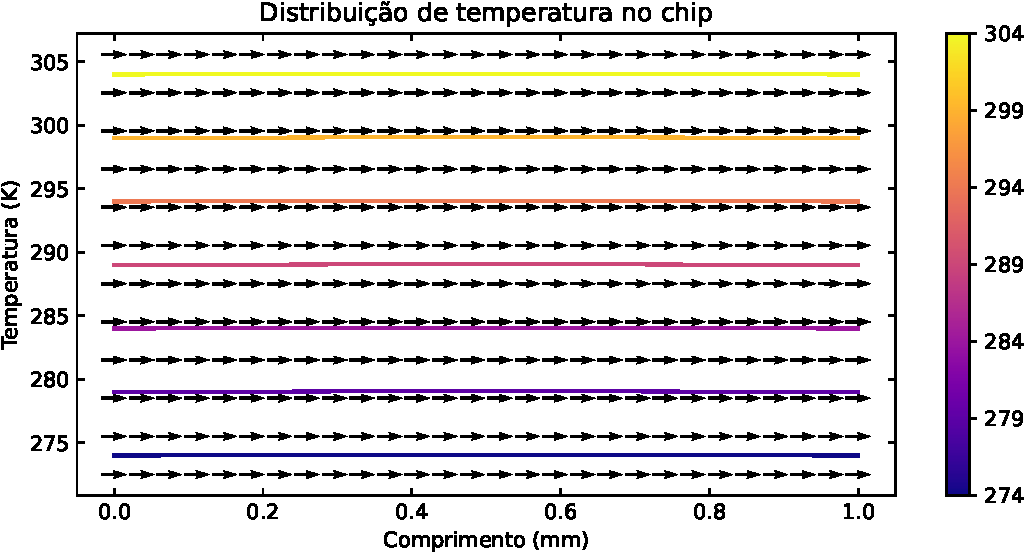
\includegraphics[width=0.9\textwidth]{../plots/val_1.pdf}
  \caption{Solução $u(x)$ com condições de contorno não homogêneas, $u(0) = u(1) = T_0$ e $T_0 \in [274, 304]$ junto do campo de tangentes normalizado}
  \label{fig:val}
\end{figure}

\begin{figure}[!ht]
  \centering
  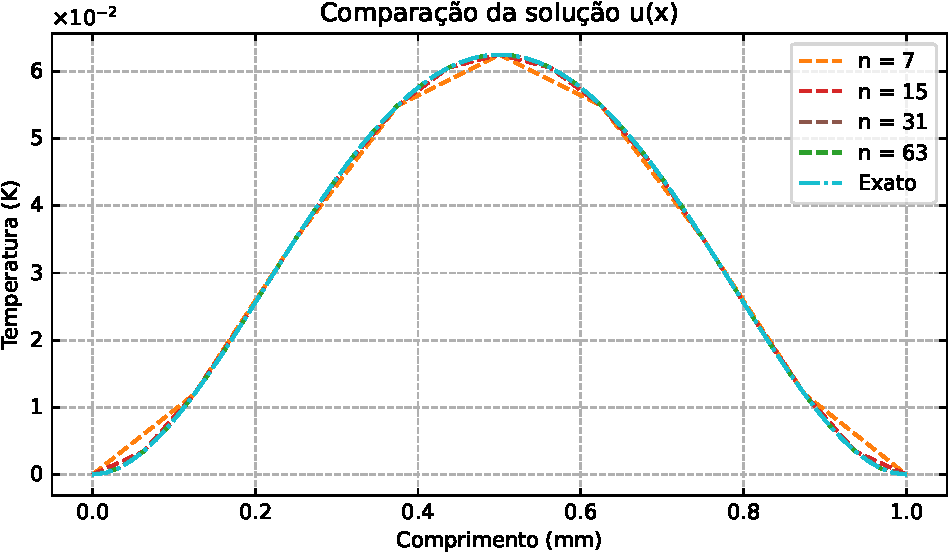
\includegraphics[width=0.78\textwidth]{../plots/val_1_comp.pdf}
  \caption{Comparação da solução calculada a partir de diferentes números de pontos interpolados com a solução exata}
  \label{fig:val_comp}
\end{figure}

\begin{figure}[!ht]
  \centering
  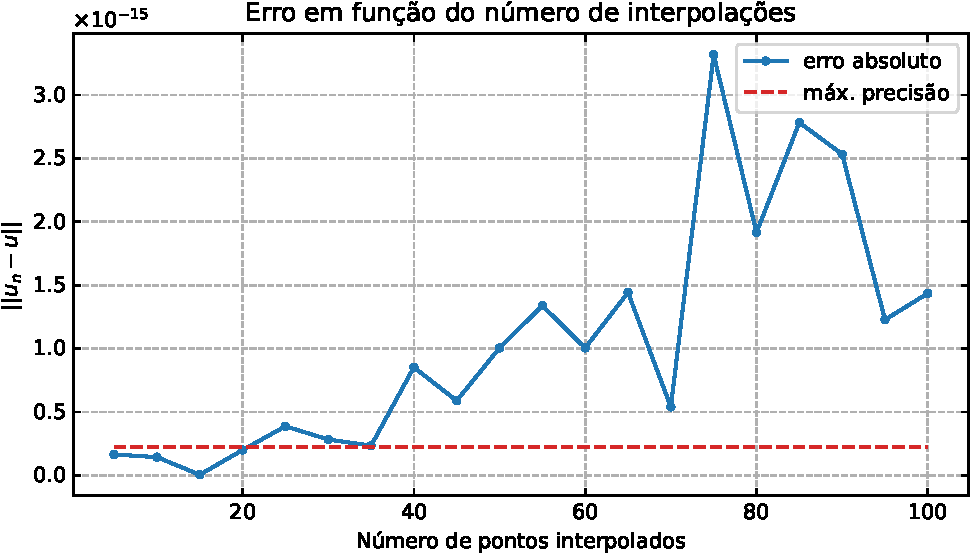
\includegraphics[width=0.8\textwidth]{../plots/val_1_err.pdf}
  \caption{Erro absoluto entre a solução aproximada $u_n$ e a solução exata $u$ para diferentes valores de $n$}
  \label{fig:val_err}
\end{figure}

\begin{table}[!ht]
  \renewcommand\arraystretch{1.45}
  \centering
  \caption{Parâmetros do modelo usado no Teste 8}
  \label{tab:convergencia}
  \doubleRuleSep
  \begin{tabular}{lrr}
    \doubleTopRule
    n  & Erro absoluto            & Ordem                   \\
    \midrule
    7  & $6.9389 \times 10^{-18}$ & -                       \\
    15 & $6.9389 \times 10^{-18}$ & 1                       \\
    31 & $1.8041 \times 10^{-16}$ & $3.8461 \times 10^{-2}$ \\
    63 & $5.6899 \times 10^{-16}$ & $3.1707 \times 10^{-1}$ \\
    \doubleBottomRule
  \end{tabular}
\end{table}


\clearpage
\subsection{Testes com forçantes de calor}
\label{sec:forcantes}
A equação diferencial \eqref{eq:estacionario} que define o sistema modelado é resolvida pelo método de Rayleigh-Ritz. Em todos os testes com forçantes de calor, é considerado $k(x) = 3.6$

\subsubsection{Teste 1}
Neste teste tanto o aquecimento quanto o resfriamento são modelados como constantes ao longo do chip. Os valores dos parâmetros deste teste estão dispostos na Tabela \ref{tab:t1_param} e o calor total do sistema é modelado pela eq. \eqref{eq:t1_q}

\begin{equation}\label{eq:t1_q}
  Q = Q^0_+ - Q^0_-
\end{equation}

\begin{table}[!ht]
  \renewcommand\arraystretch{1.45}
  \centering
  \caption{Parâmetros do modelo usado no Teste 1}
  \label{tab:t1_param}
  \doubleRuleSep
  \begin{tabular}{lr}
    \doubleTopRule
    Parâmetro                             & Valor \\
    \midrule
    Comprimento do chip ($L$)             & 20    \\
    Calor adicionado no sistema ($Q^0_+$) & 60    \\
    Calor retidado do sistema ($Q^0_-$)   & 55    \\
    \doubleBottomRule
  \end{tabular}
\end{table}

\begin{figure}[!ht]
  \centering
  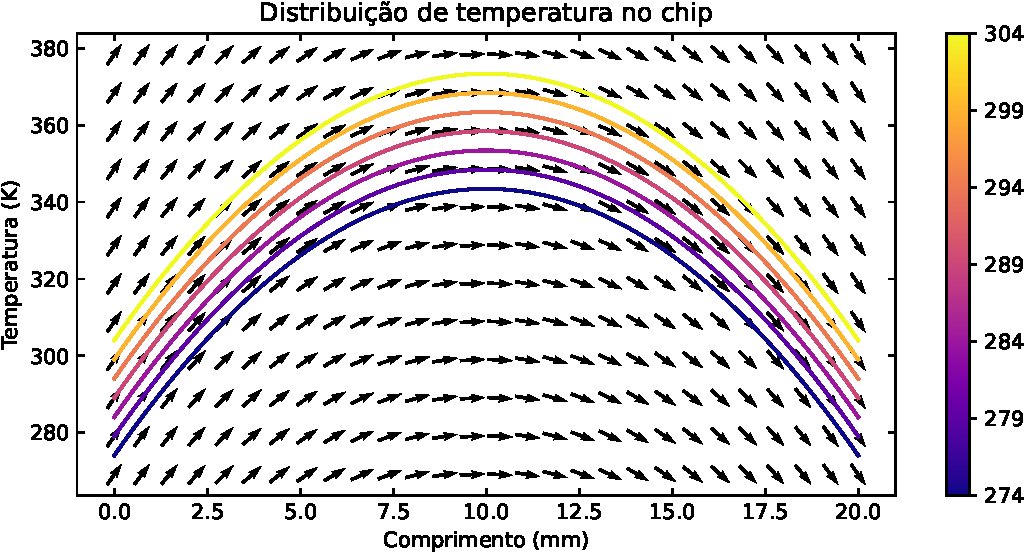
\includegraphics[width=0.9\textwidth]{../plots/test_1.pdf}
  \caption{Solução $u(x)$ com condições de contorno não homogêneas, $u(0) = u(20) = T_0$ e $T_0 \in [274, 304]$ junto do campo de tangentes normalizado}
  \label{fig:t1}
\end{figure}

\begin{figure}[!ht]
  \centering
  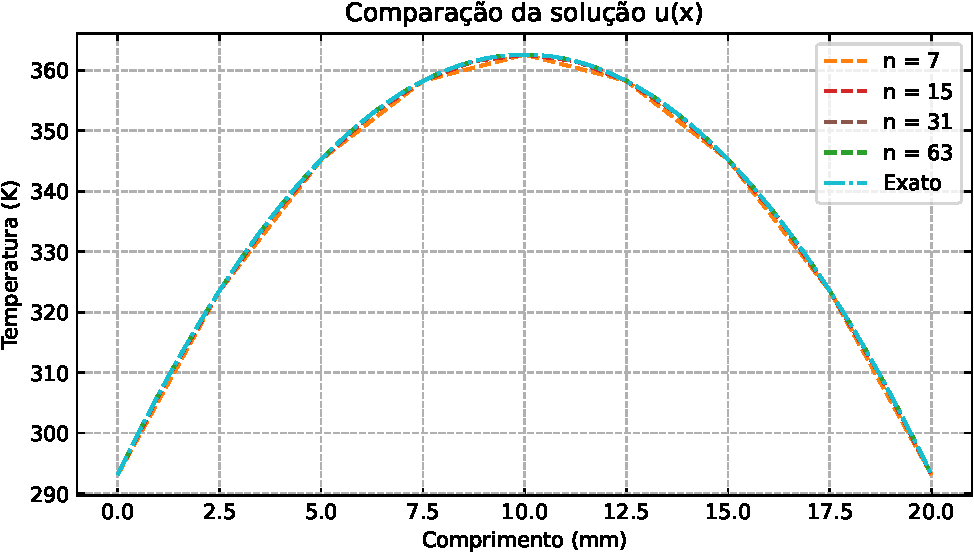
\includegraphics[width=0.9\textwidth]{../plots/test_1_comp.pdf}
  \caption{Comparação da solução calculada a partir de diferentes números de pontos interpolados com a solução exata}
  \label{fig:t1_comp}
\end{figure}

\newpage
\subsubsection{Teste 2}
Neste teste o aquecimento é modelado como uma distribuição gaussiana e o resfriamento é constantes ao longo do chip. Os valores dos parâmetros deste teste estão dispostos na Tabela \ref{tab:t2_param} e o calor total do sistema é modelado pela eq. \eqref{eq:t2_q}

\begin{equation}\label{eq:t2_q}
  Q = Q^0_+\exp\left(\frac{-\left(x-\frac{L}{2}\right)^2}{\sigma_+ ^2}\right) - Q^0_-
\end{equation}

\begin{table}[!ht]
  \renewcommand\arraystretch{1.45}
  \centering
  \caption{Parâmetros do modelo usado no Teste 2}
  \label{tab:t2_param}
  \doubleRuleSep
  \begin{tabular}{lr}
    \doubleTopRule
    Parâmetro                                                      & Valor \\
    \midrule
    Comprimento do chip ($L$)                                      & 20    \\
    Calor adicionado no sistema ($Q^0_+$)                          & 60    \\
    Calor retidado do sistema ($Q^0_-$)                            & 35    \\
    Variação de aquecimento em torno do ponto central ($\sigma_+$) & 5.5   \\
    \doubleBottomRule
  \end{tabular}
\end{table}

\begin{figure}[!ht]
  \centering
  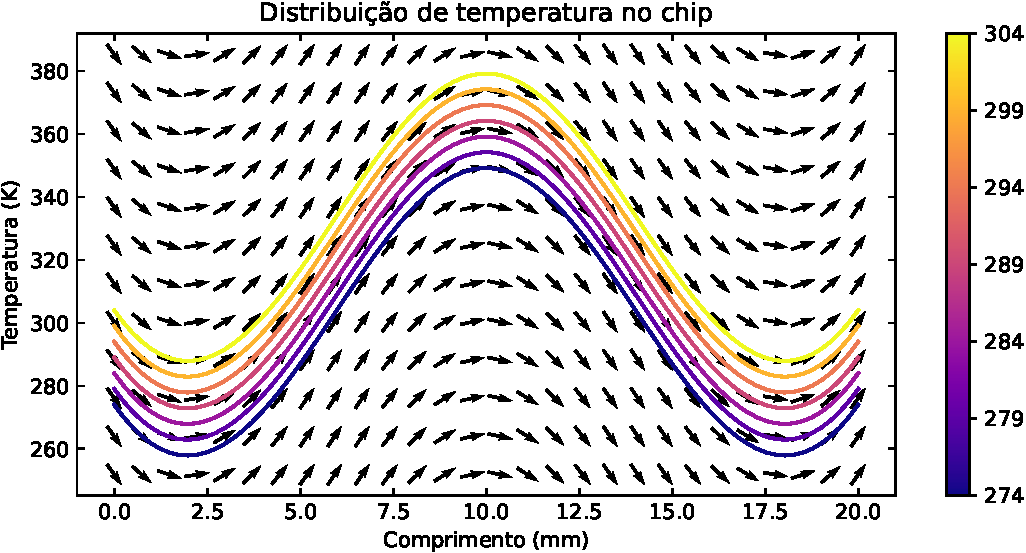
\includegraphics[width=0.9\textwidth]{../plots/test_2.pdf}
  \caption{Solução $u(x)$ com condições de contorno não homogêneas, $u(0) = u(20) = T_0$ e $T_0 \in [274, 304]$ junto do campo de tangentes normalizado}
  \label{fig:t2}
\end{figure}

\begin{figure}[!ht]
  \centering
  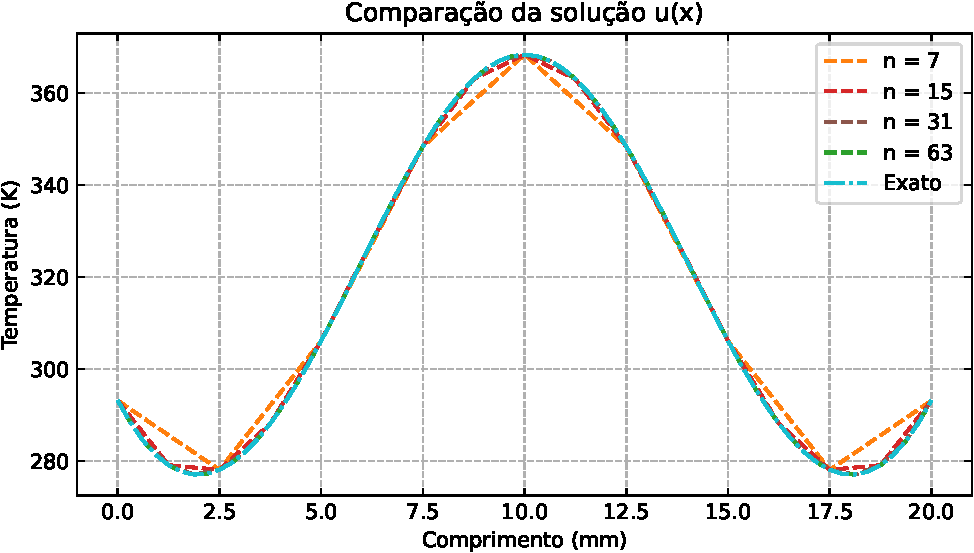
\includegraphics[width=0.9\textwidth]{../plots/test_2_comp.pdf}
  \caption{Comparação da solução calculada a partir de diferentes números de pontos interpolados com a solução exata}
  \label{fig:t2_comp}
\end{figure}

\clearpage
\subsubsection{Teste 3}
Neste teste tanto o aquecimento quanto o resfriamento são modelados como distribuição gaussiana ao longo do chip. Os valores dos parâmetros deste teste estão dispostos na Tabela \ref{tab:t3_param} e o calor total do sistema é modelado pela eq. \eqref{eq:t3_q}

\begin{equation}\label{eq:t3_q}
  Q = Q^0_+\exp\left(\frac{-\left(x-\frac{L}{2}\right)^2}{\sigma_+ ^2}\right) - Q^0_-\exp\left(\frac{-\left(x-\frac{L}{2}\right)^2}{\sigma_- ^2}\right)
\end{equation}

\begin{table}[!ht]
  \renewcommand\arraystretch{1.45}
  \centering
  \caption{Parâmetros do modelo usado no Teste 3}
  \label{tab:t3_param}
  \doubleRuleSep
  \begin{tabular}{lr}
    \doubleTopRule
    Parâmetro                                                       & Valor \\
    \midrule
    Comprimento do chip ($L$)                                       & 20    \\
    Calor adicionado no sistema ($Q^0_+$)                           & 60    \\
    Calor retidado do sistema ($Q^0_-$)                             & 60    \\
    Variação de aquecimento em torno do ponto central ($\sigma_+$)  & 3     \\
    Variação de resfriamento em torno do ponto central ($\sigma_-$) & 3     \\
    \doubleBottomRule
  \end{tabular}
\end{table}

\begin{figure}[!ht]
  \centering
  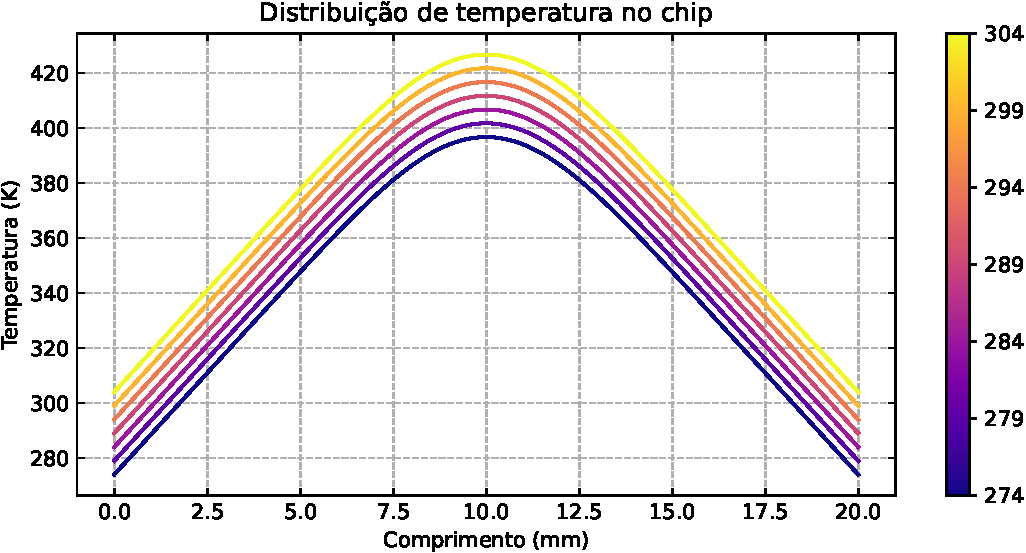
\includegraphics[width=0.9\textwidth]{../plots/test_3.pdf}
  \caption{Solução $u(x)$ com condições de contorno não homogêneas, $u(0) = u(20) = T_0$ e $T_0 \in [274, 304]$}
  \label{fig:t3}
\end{figure}

\begin{figure}[!ht]
  \centering
  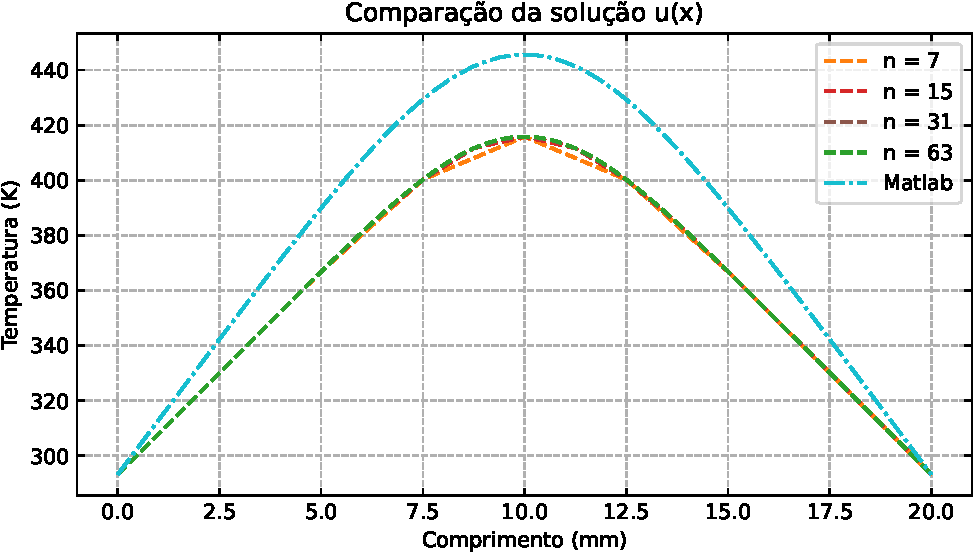
\includegraphics[width=0.9\textwidth]{../plots/test_3_comp.pdf}
  \caption{Comparação da solução calculada a partir de diferentes números de pontos interpolados com a solução obtida pelo Matlab}
  \label{fig:t3_comp}
\end{figure}

\newpage
Agora, com os mesmos parâmetros, mas considerando um resfriamento um pouco menor, $Q^0_- = 40$, chega-se a solução mostrada na Fig. \ref{fig:t3_1}

\begin{figure}[!ht]
  \centering
  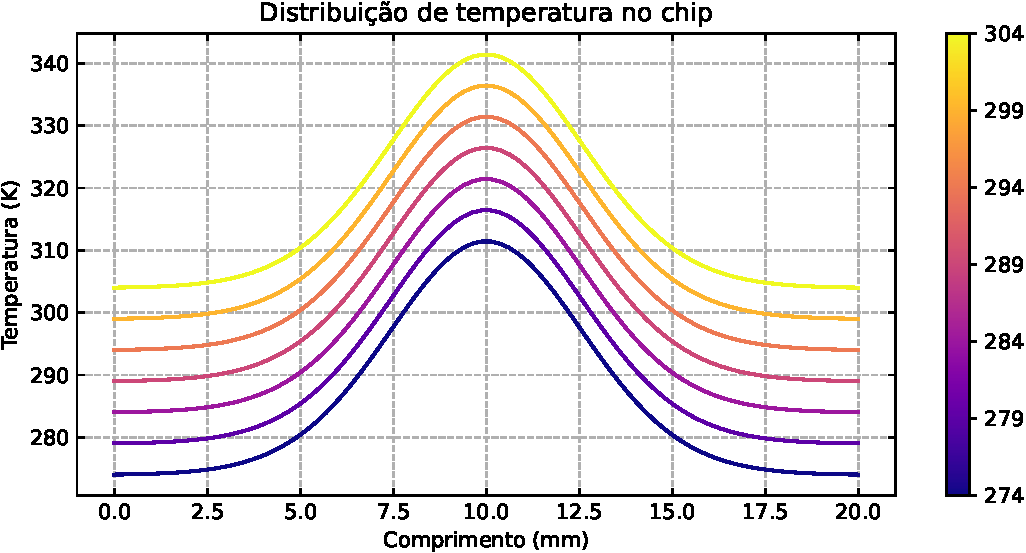
\includegraphics[width=0.9\textwidth]{../plots/test_3_1.pdf}
  \caption{Solução $u(x)$ com condições de contorno não homogêneas, $u(0) = u(20) = T_0$ e $T_0 \in [274, 304]$}
  \label{fig:t3_1}
\end{figure}


\clearpage
\subsubsection{Teste 4}
Neste teste, o aquecimento é modelado como uma distribuição gaussiana e o resfriamento é uma distribuição gaussiana mais intensa nos extremos do chip. Os valores dos parâmetros deste teste estão dispostos na Tabela \ref{tab:t4_param} e o calor total do sistema é modelado pela eq. \eqref{eq:t4_q}

\begin{equation}\label{eq:t4_q}
  Q = Q^0_+\left[\exp\left(\frac{-\left(x-\frac{L}{2}\right)^2}{\sigma_+ ^2}\right)\right] - Q^0_-\left[\exp\left(\frac{-\left(x\right)^2}{\theta ^2}\right)+\exp\left(\frac{-\left(x-L\right)^2}{\theta ^2}\right)\right]
\end{equation}

\begin{table}[!ht]
  \renewcommand\arraystretch{1.45}
  \centering
  \caption{Parâmetros do modelo usado no Teste 4}
  \label{tab:t4_param}
  \doubleRuleSep
  \begin{tabular}{lr}
    \doubleTopRule
    Parâmetro                                                      & Valor \\
    \midrule
    Comprimento do chip ($L$)                                      & 20    \\
    Calor adicionado no sistema ($Q^0_+$)                          & 60    \\
    Calor retidado do sistema ($Q^0_-$)                            & 55    \\
    Variação de aquecimento em torno do ponto central ($\sigma_+$) & 1.2   \\
    Variação de resfriamento em torno do ponto central ($\theta$)  & 2.9   \\
    \doubleBottomRule
  \end{tabular}
\end{table}

\begin{figure}[!ht]
  \centering
  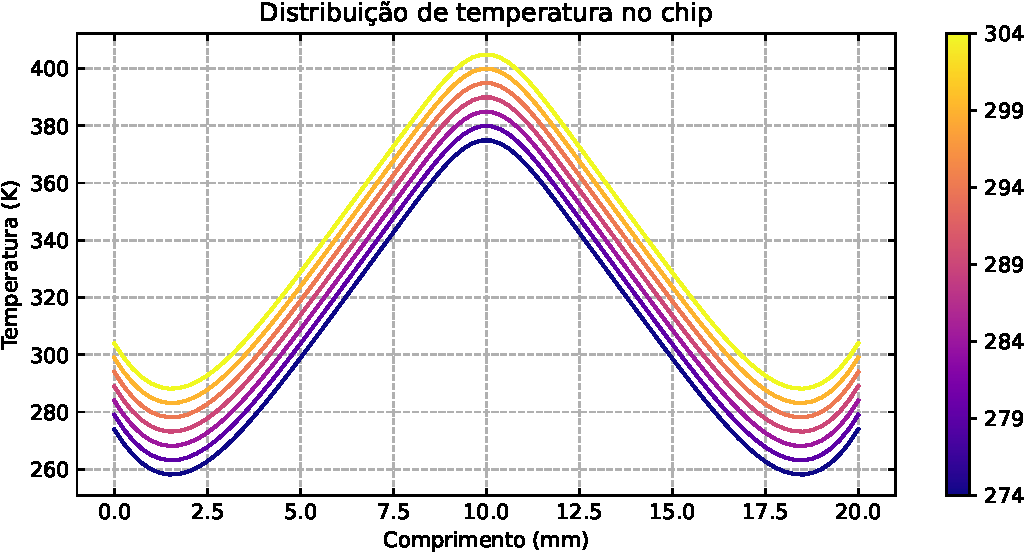
\includegraphics[width=0.9\textwidth]{../plots/test_4.pdf}
  \caption{Solução $u(x)$ com condições de contorno não homogêneas, $u(0) = u(20) = T_0$ e $T_0 \in [274, 304]$}
  \label{fig:t4}
\end{figure}

\begin{figure}[!ht]
  \centering
  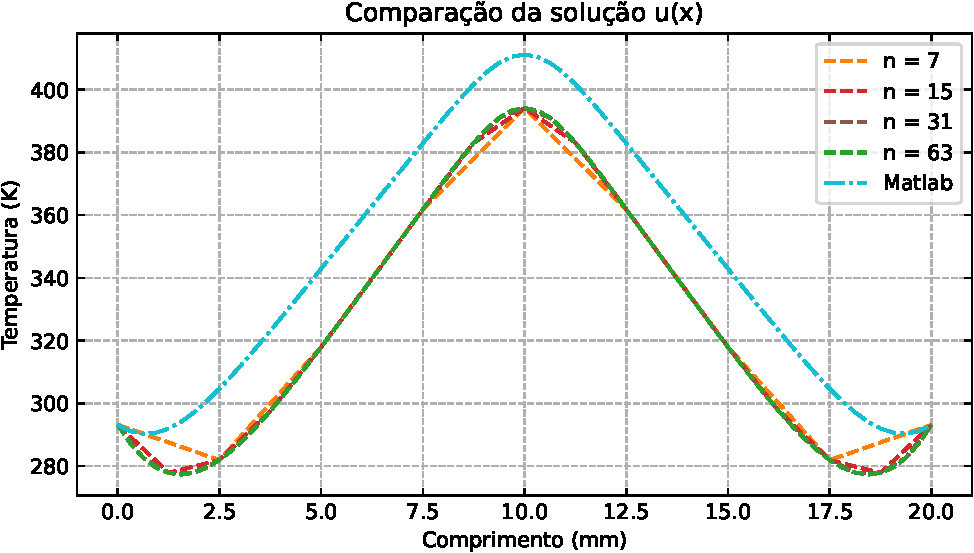
\includegraphics[width=0.9\textwidth]{../plots/test_4_comp.pdf}
  \caption{Comparação da solução calculada a partir de diferentes números de pontos interpolados com a solução obtida pelo Matlab}
  \label{fig:t4_comp}
\end{figure}

\newpage
\newpage
\subsection{Testes com variação de material}
\label{sec:variacao}
Nos testes com variação de material, $k(x)$ é descrito pela eq. \eqref{eq:var-k}

\begin{equation}\label{eq:var-k}
  k(x) = \begin{cases}k_s&\textrm{se}\:x\in \left(\frac{L}{2}-d,\:\frac{L}{2}+d\right)\\ k_a&\textrm{caso contrario}\end{cases}
\end{equation}

\newpage
\subsubsection{Teste 5}
Neste teste, tanto o aquecimento quanto o resfriamento são modelados como constantes ao longo do chip. Os valores dos parâmetros deste teste estão dispostos na Tabela \ref{tab:t5_param} e o calor total do sistema é modelado pela eq. \eqref{eq:t1_q}

\begin{table}[!ht]
  \renewcommand\arraystretch{1.45}
  \centering
  \caption{Parâmetros do modelo usado no Teste 5}
  \label{tab:t5_param}
  \doubleRuleSep
  \begin{tabular}{lr}
    \doubleTopRule
    Parâmetro                                 & Valor \\
    \midrule
    Comprimento do chip ($L$)                 & 20    \\
    Calor adicionado no sistema ($Q^0_+$)     & 60    \\
    Calor retidado do sistema ($Q^0_-$)       & 30    \\
    Condutividade térmica do silício  ($k_s$) & 3.6   \\
    Condutividade térmica do alumínio ($k_a$) & 60    \\
    \doubleBottomRule
  \end{tabular}
\end{table}

\begin{figure}[!ht]
  \centering
  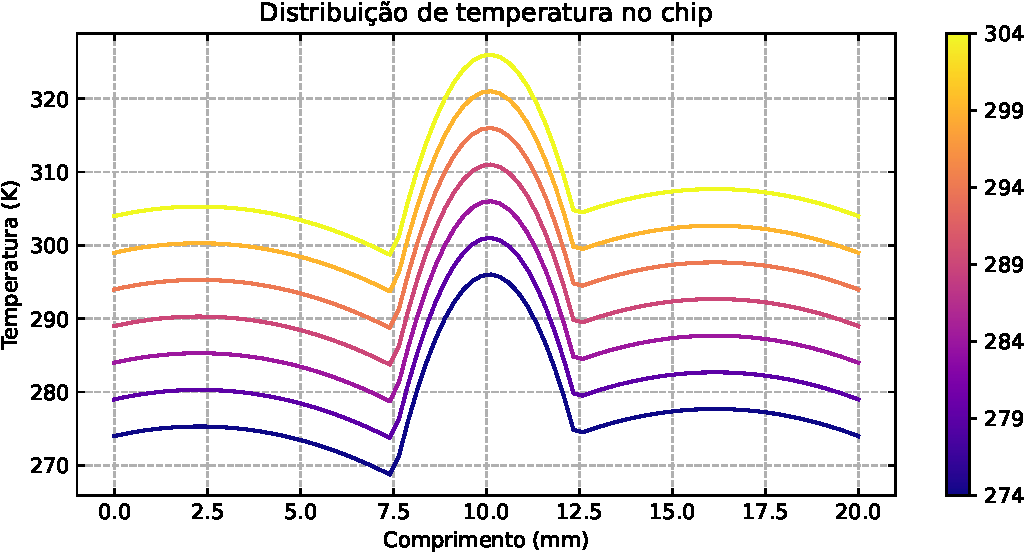
\includegraphics[width=0.9\textwidth]{../plots/test_5.pdf}
  \caption{Solução $u(x)$ com condições de contorno não homogêneas, $u(0) = u(20) = T_0$ e $T_0 \in [274, 304]$}
  \label{fig:t5}
\end{figure}

\newpage
\subsubsection{Teste 6}
Neste teste, o aquecimento é modelado como uma distribuição gaussiana e o resfriamento é constantes ao longo do chip. Os valores dos parâmetros deste teste estão dispostos na Tabela \ref{tab:t6_param} e o calor total do sistema é modelado pela eq. \eqref{eq:t2_q}

\begin{table}[!ht]
  \renewcommand\arraystretch{1.45}
  \centering
  \caption{Parâmetros do modelo usado no Teste 6}
  \label{tab:t6_param}
  \doubleRuleSep
  \begin{tabular}{lr}
    \doubleTopRule
    Parâmetro                                                      & Valor \\
    \midrule
    Comprimento do chip ($L$)                                      & 20    \\
    Calor adicionado no sistema ($Q^0_+$)                          & 60    \\
    Calor retidado do sistema ($Q^0_-$)                            & 35    \\
    Variação de aquecimento em torno do ponto central ($\sigma_+$) & 5.5   \\
    Condutividade térmica do silício  ($k_s$)                      & 3.6   \\
    Condutividade térmica do alumínio ($k_a$)                      & 60    \\
    \doubleBottomRule
  \end{tabular}
\end{table}

\begin{figure}[!ht]
  \centering
  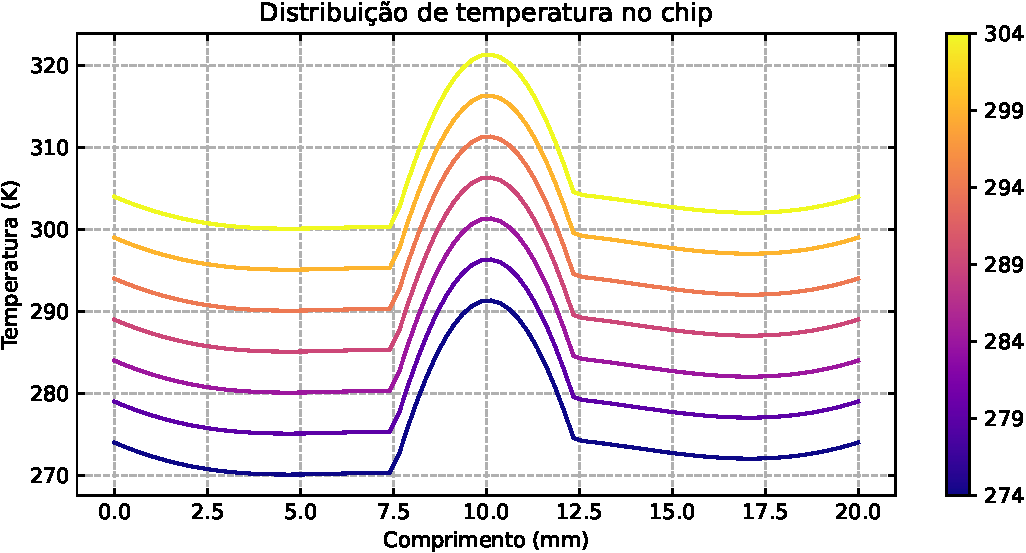
\includegraphics[width=0.9\textwidth]{../plots/test_6.pdf}
  \caption{Solução $u(x)$ com condições de contorno não homogêneas, $u(0) = u(20) = T_0$ e $T_0 \in [274, 304]$}
  \label{fig:t6}
\end{figure}

\newpage
\subsubsection{Teste 7}
Neste teste, tanto o aquecimento quanto o resfriamento são modelados como distribuição gaussiana ao longo do chip. Os valores dos parâmetros deste teste estão dispostos na Tabela \ref{tab:t7_param} e o calor total do sistema é modelado pela eq. \eqref{eq:t3_q}

\begin{table}[!ht]
  \renewcommand\arraystretch{1.45}
  \centering
  \caption{Parâmetros do modelo usado no Teste 7}
  \label{tab:t7_param}
  \doubleRuleSep
  \begin{tabular}{lr}
    \doubleTopRule
    Parâmetro                                                       & Valor \\
    \midrule
    Comprimento do chip ($L$)                                       & 20    \\
    Calor adicionado no sistema ($Q^0_+$)                           & 60    \\
    Calor retidado do sistema ($Q^0_-$)                             & 30    \\
    Variação de aquecimento em torno do ponto central ($\sigma_+$)  & 2     \\
    Variação de resfriamento em torno do ponto central ($\sigma_-$) & 8     \\
    Condutividade térmica do silício  ($k_s$)                       & 3.6   \\
    Condutividade térmica do alumínio ($k_a$)                       & 60    \\
    \doubleBottomRule
  \end{tabular}
\end{table}

\begin{figure}[!ht]
  \centering
  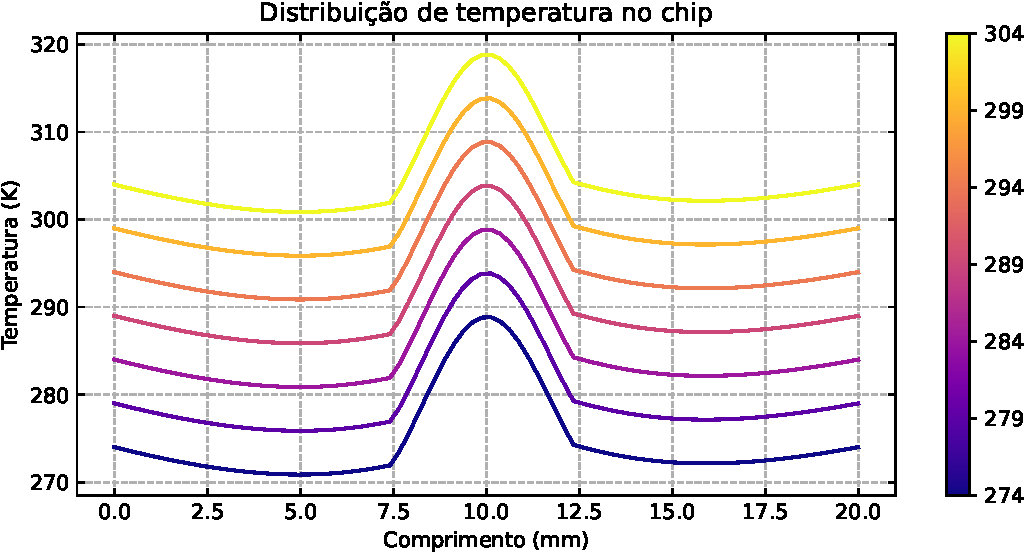
\includegraphics[width=0.9\textwidth]{../plots/test_7.pdf}
  \caption{Solução $u(x)$ com condições de contorno não homogêneas, $u(0) = u(20) = T_0$ e $T_0 \in [274, 304]$}
  \label{fig:t8}
\end{figure}


\newpage
\subsubsection{Teste 8}
Neste teste, o aquecimento é modelado como uma distribuição gaussiana e o resfriamento é uma distribuição gaussiana mais intensa nos extremos do chip. Os valores dos parâmetros deste teste estão dispostos na Tabela \ref{tab:t8_param} e o calor total do sistema é modelado pela eq. \eqref{eq:t4_q}

\begin{table}[!ht]
  \renewcommand\arraystretch{1.45}
  \centering
  \caption{Parâmetros do modelo usado no Teste 8}
  \label{tab:t8_param}
  \doubleRuleSep
  \begin{tabular}{lr}
    \doubleTopRule
    Parâmetro                                                      & Valor \\
    \midrule
    Comprimento do chip ($L$)                                      & 20    \\
    Calor adicionado no sistema ($Q^0_+$)                          & 60    \\
    Calor retidado do sistema ($Q^0_-$)                            & 30    \\
    Variação de aquecimento em torno do ponto central ($\sigma_+$) & 2     \\
    Variação de resfriamento em torno do ponto central ($\theta$)  & 4     \\
    Condutividade térmica do silício  ($k_s$)                      & 3.6   \\
    Condutividade térmica do alumínio ($k_a$)                      & 60    \\
    \doubleBottomRule
  \end{tabular}
\end{table}

\begin{figure}[!ht]
  \centering
  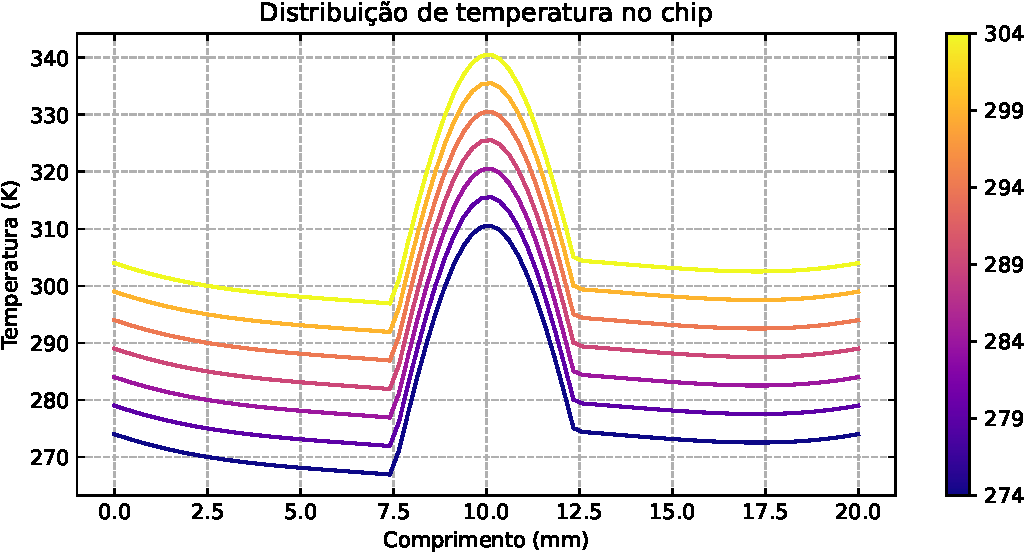
\includegraphics[width=0.9\textwidth]{../plots/test_8.pdf}
  \caption{Solução $u(x)$ com condições de contorno não homogêneas, $u(0) = u(20) = T_0$ e $T_0 \in [274, 304]$}
  \label{fig:t8}
\end{figure}


\newpage
\section{Conclusão}
Neste trabalho, projetamos um sistema de resfriamento de chips partindo da abstração do problema físico, levantamento de hipóteses e simplificações (Seção \ref{sec:modelagem}), passando pela descrição do método de Rayleigh-Ritz utilizado para resolver o problema (Seção \ref{sec:rr}) e respectivas otimizações de implementação deste método (Seção \ref{sec:design}) até a analise dos resultados obtidos (Seções \ref{sec:validacao}, \ref{sec:forcantes} e \ref{sec:variacao}).

Os resultados obtidos pelos testes quando comparados com o valor exato ou com o valor obtido por simulação no Matlab são bem próximos. Com isso, concluímos que o método de Rayleigh-Ritz eficaz para resolver o problema proposto, tendo grande eficácia em obter a aproximação da solução da equação diferencial.

% \vspace{10mm}

% \section*{Apêndice}
% \appendix


\bibliographystyle{plainnat}
\bibliography{refs}

\horizonBackCover
\end{document}
